\section{Theory behind the Pockels effect}

\subsection{Light propagating in matter}
\paragraph{The basis of discussing} 
electro-optical effects are 
Maxwell's equations in matter~\cite{boyd2003nonlinear}:
\begin{subequations} 
\begin{align}
\nabla \cdot \D &= \rho_\text{f} 
\label{eq:max1} \\ 
\nabla \cdot \B &= 0
\label{eq:max2} \\ 
\nabla \times \E &= -\frac{\partial \B} {\partial t}
\label{eq:max3} \\ 
    \nabla \times \mathbf{H} &= \mathbf{J}_\text{f} + 
        \frac{\partial \D} {\partial t}, 
\label{eq:max4}
\end{align}
\label{eq:maxwell}
\end{subequations}
where 
\begin{itemize}
    \item $\D$ is the electric displacement field, related to the eletric field $\E$ 
    by the constitutive equation 
    \begin{equation}
        \D = \Eps \E 
    \label{eq:const1}
    \end{equation}
    where $\Eps$ is the dielectric tensor;
    \item $\mathbf{H}$ is the magnetizing field, with the constitutive equation 
    \begin{equation}
        \mathbf{H} = \mu^{-1} \, ;
    \label{eq:const2}
    \end{equation}
    \item $\mathbf{J}_\text{f}$ is the free current density, and
    \item $\mathbf{\rho}_\text{f}$ is the free charge density.
\end{itemize}
Equations \eqref{eq:const1} and \eqref{eq:const2} are valid for materials without 
coupling between magnetic and eletric fields, which is the case in our 
crystal. We are, however, facing an anistropic material, so that 
$\Eps$ is a tensor, while we assume the permeability $\mu$ of the material 
to be just the vacuum permeability $\mu_0$, such that
$\B = \mu \mathbf{H} = \mu_0 \mathbf{H}$. 
If we assume $\mathbf{\rho}_\text{f} = 0$, $\mathbf{J}_\text{f} = 0$ 
(no free charge and currents), we obtain the homogenious 
Maxwell equations. By applying the curl operator $\nabla \times$ 
to \eqref{eq:max3}, we get the wave equation 
\begin{equation}
    - \Delta \E + \frac{\eps}{\epsn c^2} \frac{\partial^2 \E}{\partial t^2}  = 0
    \label{eq:wave_eq}
\end{equation}
which possesses plane waves as solutions, 
described by
\begin{subequations}
\begin{align}
    \E &= \E_0 \exp \left[i(\mathbf{k \cdot r}-\omega t)\right] \\
    \mathbf{H} &= \mathbf{H_0} \exp \left[i(\mathbf{k \cdot r}-\omega t)\right], 
\end{align}
\end{subequations}

Inserting into \eqref{eq:max3} and \eqref{eq:max4} yields:
\begin{subequations}
\begin{align}
    \mu_0 \omega \mathbf{H} &= \K \times \E 
    \label{eq:plan_H} \\
    \omega \D &= - \K \times \mathbf{H}.
    \label{eq:plan_D} 
\end{align}
\end{subequations}
We observe, that $\K, \D$, and $\Ha$ are mutually perpendicular. 
Looking at the energy flux
\begin{equation}
    \mathbf{S} = \E \times \Ha, 
\end{equation}
we further see, that the directions of $\mathbf{S}$ and $\K$ do not 
coincide if $\E \nparallel \Eps \E$. 

\paragraph{As a consequence}, 
plane waves can be polarized in any direction 
perpendicular to $\K$. Linear polarized waves conserve the 
direction of polarization in time and space. They are formed 
the superposing two waves with the same frequency and a 
relative phase $\Delta \phi = n \pi$, where $n \in \mathbb{Z}$. 
Any linearly polarized wave can be split up into two orthogonal 
components of equal amplitude, each forming an angle of $45^\circ$ 
with the original polarization.
A linear combination of two aves of the same frequency $\omega$, 
wavevector $\K$ but orthogonal polarization and a fixed phase 
difference $\Delta \phi \neq 0$ is generally polarized elliptically.
For the special case of equal amplitudes and $\Delta \phi = \pi /2$,
the polarization is circular. 

\paragraph{In order to asses} 
the differences in phase induces by the Pockels effect, we need to 
relate refraction to the phase. To do so, we look at two plane waves  
\begin{align}
\E_1(\mathbf{r}, t) = (\E_1)_0 \exp\left\{i(\K_1 \cdot \mathbf{r} - \omega t) \right\} \\ 
\E_2(\mathbf{r}, t) = (\E_2)_0 \exp\left\{i(\K_2 \cdot \mathbf{r} - \omega t) \right\} \\ 
\end{align}
with the same frequency $\omega$,
we can define $\Delta \phi$ at 
one time $t$ and position $\mathbf{r}$ by 
\begin{equation}
    \Delta \phi := \left(\K_2 - \K_1 \right) \cdot \mathbf{r}\, .
\end{equation}
By the definition of $\N$ \eqref{eq:def_n} and the identity 
\begin{equation}
    \omega = \frac{2 \pi c}{\lambda} \, ,
\end{equation}
we can write 
\begin{equation}
    \Delta \phi = \frac{2 \pi}{\lambda} 
    \left(\N_2 - \N_1 \right) \cdot \mathbf{r} \, .
\end{equation}
If we further assume $\N$ to be parallel to $\mathbf{r}$, 
and measure $\Delta \phi$ after the two waves passed 
through a crystal of lenght $l$, then we get
\begin{equation}
    \Delta \phi_l = \frac{2 \pi}{\lambda} 
    \left(n_2 - n_1 \right) l \, .
    \label{eq:dphi}
\end{equation}


\subsection{Birefringence}
\paragraph{If the refraction index}
 $n$ of a material depends on the linear polarization of light, 
then a beam of light propagating in the material will be split up into 
two beams with perpendicular polarization and different propagation speed 
\begin{equation}
   v_i = \frac{c}{n_i}, 
\end{equation}
In order to explain this phenomenon, it is helpful to examine the 
structure of the material and connected quantities, as well as 
to retrieve the way light propagates by looking at the solutions 
of Maxwell's equations in matter \eqref{eq:maxwell}.
If we define the 
refractive index $\mathbf{n}$ by 
\begin{equation}
    \K = \frac{\omega}{c} \N \, ,
    \label{eq:def_n}
\end{equation}
we can rewrite equations \eqref{eq:plan_H} and \eqref{eq:plan_D} as 
\begin{subequations}
\begin{align}
    \mathbf{H} &= \frac{1}{\mu_0 c} \N \times \E 
    \label{eq:plan_Hb} \\
    \D &= - \frac{1}{c} \N \times \mathbf{H}
    \label{eq:plan_Db} \, .
\end{align}
\end{subequations}
Inserting the latter one into the first and using 
the identity $c^2 = \frac{1}{\mu_0 \epsn}$, we get 
\begin{equation}
    \begin{split}
    \D  &= \frac{1}{\mu_0 c^2} \N \times \left(\E \times \N\right) \\
        &= \epsn \left(n^2 \E - \left(\N \cdot \E\right) \N \right)
    \label{eq:D(E)}
    \end{split}
\end{equation}
With the constitutive equation \eqref{eq:const1}, we obtain three 
equations linear in the components $E_k$:
\begin{equation}
    \left(n^2 \delta_{ik} - n_i n_k - \frac{\epsilon_{ik}}{\epsn}\right) E_k = 0
\end{equation}
This equation is solve if its determinant vanishes:
\begin{equation}
    \mathrm{det}\,\left|n^2 \delta_{ik} - n_i n_k - \frac{\epsilon_{ik}}{\epsn}\right| = 0
\end{equation}
By applying the principle axis theorem~\cite{strang2003introduction}, 
we can write $\Eps$ as the diagonal matrix with elements $\eps_x, \eps_y, \eps_z$. 
This yields \emph{Fresnel's equation}:
\begin{align}
    \frac{n^2}{\epsn} \left(\eps_x n_x^2 + \eps_y n_y^2 + \eps_z n_z^2 \right) 
    - \left[
        \frac{n_x^2}{\epsn^2} \eps_x \left(\eps_y + \eps_z\right) + 
        \frac{n_y^2}{\epsn^2} \eps_y \left(\eps_z + \eps_x\right) + 
        \frac{n_z^2}{\epsn^2} \eps_z \left(\eps_x + \eps_y\right) 
    \right] + \nonumber \\
    + \quad \frac{\eps_x \eps_y \eps_z}{\epsn^3} = 0
    \label{eq:fresnel}
\end{align}
Being of second order in $n_i^2$, $i \in \{x, y, z\}$, there are up to two linearly 
independent solutions, corresponding to two possible directions of polarization. 


\paragraph{The case of a uniaxial crystal} 
is especially easy to solve. 
If we take the $z$-axis to be that of rotational symmetry, 
we can rename the components of 
$\Eps$ with 
\begin{align}
\eps_x &= \eps_y = \eps_\perp 
\label{eq:eps_perp}\\
\eps_z &= \eps_\parallel \, .
\label{eq:eps_parallel}
\end{align}
The $z$-axis is also called the \emph{optical axis}.
Fresnel's equation \eqref{eq:fresnel} can then be factored into
\begin{equation}
    \left(n^2 - \frac{\eps_\perp}{\epsn}\right) 
    \left[\frac{\eps_\parallel}{\epsn} n_z^2 + 
        \frac{\eps_\perp}{\epsn} \left(n_x^2 + n_y^2\right) -
        \frac{\eps_\perp \eps_\parallel}{\epsn^2} 
    \right] = 0 \, .
\end{equation}
In other words, we have two quadratic equations
\begin{align}
    n^2 &= \frac{\eps_\perp}{\epsn} 
    \label{eq:sphere} \\
    n_z^2 \frac{\epsn}{\eps_\perp} + \left(n_x^2 + n_y^2\right) \frac{\epsn}{\eps_\parallel} &= 1
    \label{eq:ellipsoid}
\end{align}
Equation \eqref{eq:sphere} gives a sphere for the wave-vector surface. To the 
corresponding types of waves, the crystal behaves like an isotropic body, being 
characterized by the refractive index $n = \sqrt{\eps_\perp / \epsn}$. These waves are 
called \emph{ordinary waves}. The second type, accordingly named 
\emph{extraordinary waves}, is confined by the ellipsoid \eqref{eq:ellipsoid}. 
It's magnitude depends on 
the angle $\theta$ to the optical axis by 
\begin{equation}
    \frac{1}{n^2} = \epsn \left( \frac{\sin^2 \theta}{\eps_\parallel} - 
        \frac{\cos^2 \theta}{\eps_\perp} \right)\, .
    \label{eq:theta}
\end{equation}

\paragraph{In order to relate} 
these two surfaces to two directions of polarization and 
determine the direction of a ray, we introduced the \emph{ray vector} $\mathbf{s}$, 
which is defined by the direction of the group velocity
\begin{equation}
    \frac{\partial \omega}{\partial \K}
\end{equation}
and the magnitude fullfilling 
\begin{equation}
    \mathbf{s} \cdot \N = 1\,.
\end{equation}
The ray vector defines the \emph{ray surface} by the condition 
$\phi = \mathrm{const.}$ 
for all $\mathbf{s}$ on that surface, where $\phi$ is the phase of the wave. 

We can show that $\mathbf{s} \parallel \mathbf{S}$: Differentiating 
equations \eqref{eq:plan_Hb} and \eqref{eq:plan_Db}, we get 
\begin{subequations}
\begin{align}
    c \delta \D &= \delta \Ha \times \N + \Ha \times \delta \N \\
    \mu_0 c \delta \Ha &= \N \times \delta \E + \delta \N \times \E \, ,
\end{align}
\end{subequations}
which by multiplying with $\E$ and $\Ha$, respectively, and applying 
basic properties of vector and scalar products, yield
\begin{subequations}
\begin{align}
    \begin{split}
    c \E \cdot \delta \D 
    &= \E \cdot \left(\delta \Ha \times \N \right) + 
        \E \cdot \left(\Ha \times \delta \N \right) \\
    &= \delta \Ha \cdot \left(\N \times \E \right) + 
        \delta \N \cdot \left(\E \times \Ha \right)  \\
    &= \mu_0 c \Ha \cdot \delta \Ha + 
        \delta \N \cdot \left(\E \times \Ha \right)
    \end{split} \\
    \mu_0 c \Ha \cdot \delta \Ha &= c \D \cdot \delta \E + 
        \delta \N \cdot \left(\E \times \Ha \right) \, ,
\end{align}
\end{subequations}
using again \eqref{eq:plan_Hb} and \eqref{eq:plan_Db}. It follows directly, that 
\begin{equation}
    \delta \N \cdot \left( \E \times \Ha \right) = \delta \N \cdot \mathbf{S} = 0 \, .
\end{equation}
To show, that $\se$ and $\mathbf{S}$ have the same direction, we need to show, 
that $\se$ is orthogonal on the surface of the wave vector surface, or, since 
the infinitesimal displacement $\delta \N$ lies 
on that surface, that $\se \cdot \delta \N = 0$. 
The wave vector surface given by \eqref{eq:fresnel} can be described by 
$f(\omega, \K) = 0$, which implies 
\begin{equation}
    \frac{\partial \omega}{\partial \K} = 
    - \frac{\partial f / \partial \K}{\partial f / \partial \omega}
\end{equation}
for the group velocity and thus 
\begin{equation}
    \se \parallel \frac{\partial f }{\partial \K} \parallel \frac{\partial f}{\partial \N}
    \label{eq:s_dir}
\end{equation}
since the gradient along $\K$ is taken for constant $\omega$. $\partial f / \partial \N$, however, 
is normal to the surface $f = 0$, so we can conclude, that
\begin{align}
    \se \cdot \delta \N &= 0 \\
    \Rightarrow \qquad \se &\parallel \mathbf{S} \, .
\end{align}
If follows, that 
\begin{equation}
    \se \cdot \Ha = 0 \qquad \se \cdot \E = 0 \, .
    \label{eq:coplanar}
\end{equation}
For uniaxial crystals, we can specify the ray surface in a form similar to 
\eqref{eq:ellipsoid} by doing analoge calculations with the folloing substitutions:
\begin{equation}
    \E \leftrightarrow c \D \, ; 
    \qquad \N \leftrightarrow \mu_0 c \se \, ; 
    \qquad \eps_{ik} \leftrightarrow {\eps^{-1}}_{ik} \, .
\end{equation}
The result is 
\begin{align}
    s^2 &= \frac{\epsn}{\eps_\perp}
    \label{eq:s_sphere} \\
    {s_z}^2 \frac{\eps_\perp}{\epsn} + \left( {s_x}^2 + 
        {s_y}^2\right) \frac{\eps_\parallel}{\epsn} &= 1 \, .
    \label{eq:s_ellipsoid}
\end{align}
Since $\eps_x = \eps_y$, $\N$ and $\se$ must be coplanar with the optical axes. This 
common plane is called \emph{principal axis} for a given $\N$. Let this plane be 
defined by the $xz$-plane. We can get the direction 
of $\se$ from the relation \eqref{eq:s_dir}, namely by taking the derivatives of 
\eqref{eq:ellipsoid} with respect to $n_x$ and $n_z$:
\begin{equation}
    \frac{s_x}{s_z} = \frac{\eps_\perp n_x}{\eps_\parallel n_z} \, .
\end{equation}
The angle $\theta'$ between optical axis and ray vector is given in terms of 
$\theta$, as defined in equation \eqref{eq:theta}:
\begin{equation}
    \tan \theta' = \frac{\eps_\perp}{\eps_\parallel} \tan \theta\, .
\end{equation}
We observe, that the directions of $\N$ and $\se$ aor only the same for 
$\theta = m \pi / 2$, $m \in \mathbb{Z}$, 
thus for waves propagating parallel or perpendicular to the optical axis. 


\paragraph{The polarization} is analyzed taking yet another direction: 
Instead of describing the wave vector surface in principle axis 
coordinates of $\eps$, we can use coordinates corresponding to 
the fact, the $\D$ is transverse to $\N$. Taking one axis to be 
parallel to $\N$, we denote the other two directions with Greek letters. 
For the components of $\D$, we get from equation \eqref{eq:D(E)}
\begin{equation}
    D_\alpha = \epsn n^2 E_\alpha
\end{equation}
and with the constitutive equation \eqref{eq:const1} 
\begin{equation}
    E_\alpha = {\eps^{-1}}_{\alpha \beta} D_\beta \, 
\end{equation}
we get the two dimensional eigenvalue problem
\begin{equation}
    {\eps^{-1}}_{\alpha \beta} D_\beta = \epsn^{-1} n^{-2} D_\beta \,
\end{equation}
for the two-dimensional symmetric tensor $\eps^{-1}$. 
In the case of no degeneracy, we obtain two orthogonal eigenvectors 
$\D_1$ and $\D_2$. Degeneracy is only present, if the components of 
$\eps^{-1}$ are all the same in its own principla axis coordinate system - 
this would just be the case of isotropic materials. 


\paragraph{We unite the results} of the foregoing anaylsis with the 
following conclusion: 
$\N, \se, \E$ and $\D$ are always coplanar. For extraordinary waves, 
$\N$ and $\se$ are not parallel, but in the same principal section. 
The wave is thus polarized such that $\E$ and $\D$ lie in that principal 
section. As $\D$ for the ordinary waves of the same $\N$ as perpendicular 
to that of the extraordinary, their polarization is such that 
$\E$ and $\D$ are perpendicular to the principal section. 

\paragraph{For biaxial crystals,}
 the solutions are more complicated and 
treated for example in \cite{landau1984electrodynamics}. 
The fourth order surface defined by Fresnel's equation 
\eqref{eq:fresnel} can now be separated into 
two ellipsoids: There are no more ordinary rays, but only 
extraordinary ones. We can find two 
optical axes as point of self intersection of the 
surface, usually obtainted by looking at the intersections 
the the coordinate planes in the principla axis basis.
In order to do so, we set to zero one of the components 
in Fresnel's equation \eqref{eq:fresnel}. For the 
$xy$-plane, we set $n_z = 0$ and obtain
\begin{equation}
    \left(n^2 - \frac{\eps_z}{\epsn}\right) 
    \left(\frac{\eps_x}{\epsn} n_x^2 + 
        \frac{\eps_y}{\epsn} n_x^2  -
        \frac{\eps_x \eps_y}{\epsn^2} 
    \right) = 0 \, .
\end{equation}
with the solutions
\begin{align}
    n^2 &= \frac{\eps_z}{\epsn} 
    \label{eq:sphere} \\
    {n_x}^2 \frac{\epsn}{\eps_y} + {n_y}^2 \frac{\epsn}{\eps_x} &= 1
    \label{eq:ellipsoid}
\end{align}
and the analogues for $n_y = 0$ and $n_x = 0$, obtained by 
interchanging $x, y$ and $z$. If we assume 
\begin{equation}
    \eps_z > \eps_y > \eps_x, 
\end{equation}
we see that the intersects appear only in the $xz$-plane, as shown in 
figure \ref{fig:biaxial_ellipsoid}.
\begin{figure}
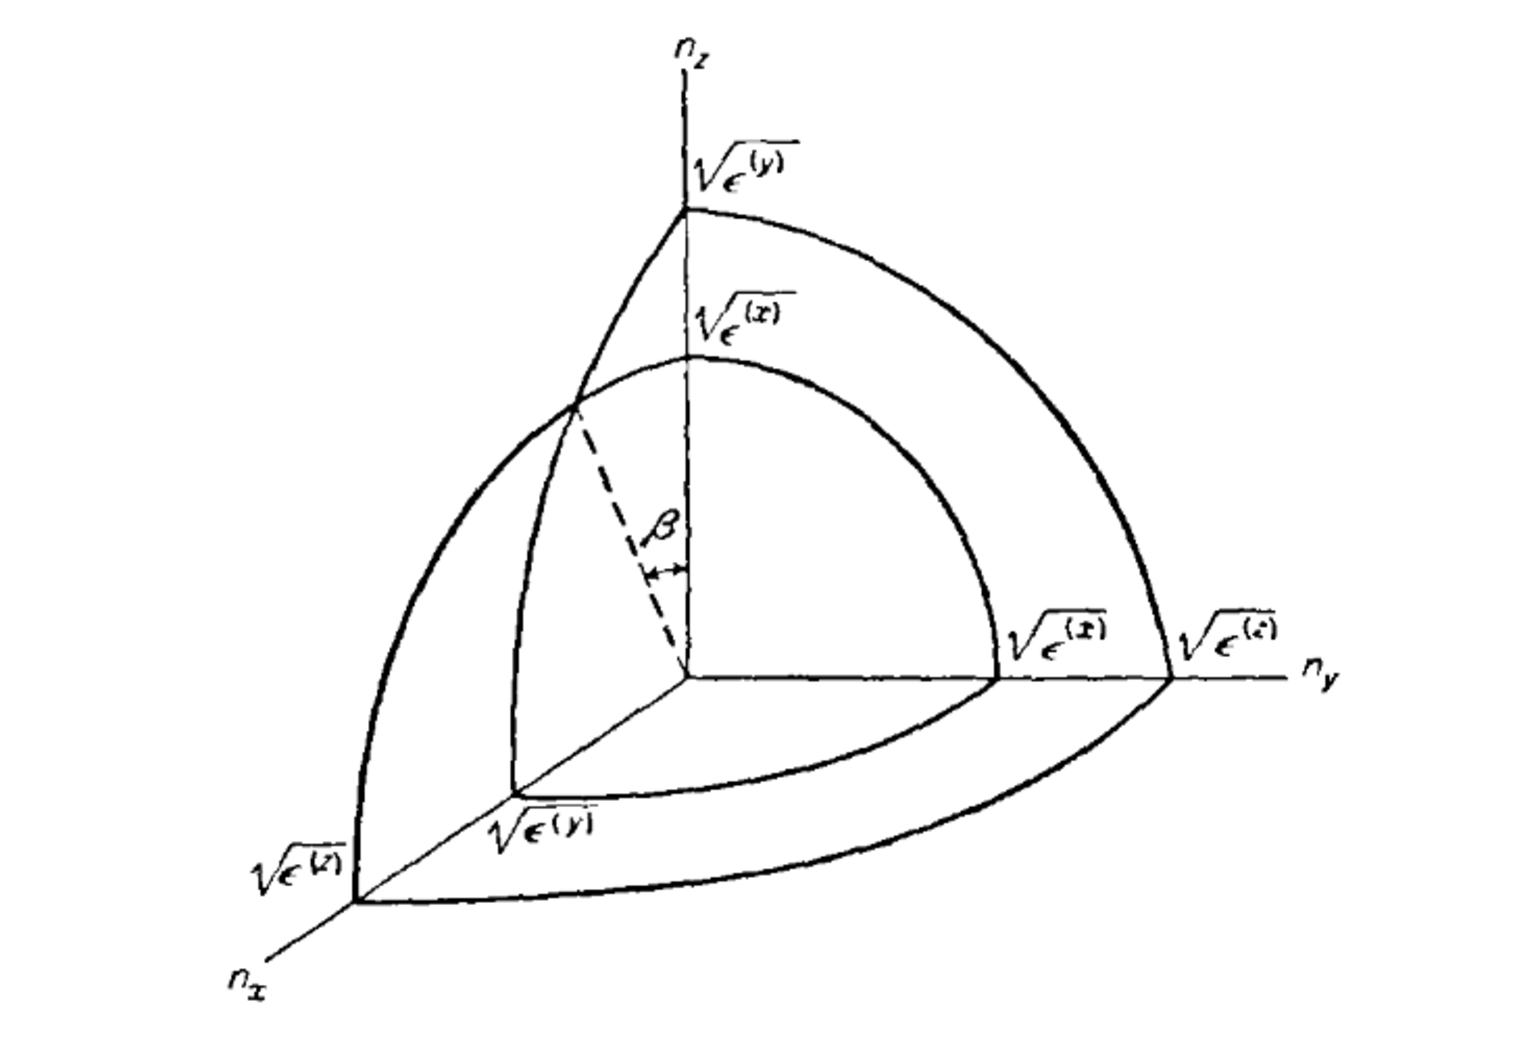
\includegraphics[width=\pltw]{figures/biaxial_ellipsoid.pdf}
\caption{Surface defined by Fresnel's equation for biaxial crystals.
    The lines are shown only on the planes parallel to the principle 
    axis of the crystal. The point of intersection defines the optical axis, 
    shown as a dashed line. 
    Taken from \cite{landau1984electrodynamics}. }
\label{fig:biaxial_ellipsoid}
\end{figure}
The optical axes are now defined by the straight lines intersecting 
the self intersects of the surface and the origin. 
Wave vector $\K$ and ray vector $\se$ have the same direction, 
only if they are orientated along one of the principle axes, 
otherwise they split up into two rays. 
Further, if $\K$ lies in one of the coordinate planes, so does $\se$.
There is, however an important exception: If the wave vector 
coincides with one of the optical axes, there are 
infinitely many ray vectors associated with it:
be can observe the phenomenon of 
\emph{internal conical refraction}. 
\FloatBarrier

\subsection{Primary and secondary electro-optic effect}
\paragraph{The electro-optic tensor}
can be splitted into two components:
The primary electro-optic effect with coefficient $r_{ij}'$
for the case of zero strain, where the crystal is 
not able to deform. The secondary effect corresponds to deformation 
due to photoelastic and piezoelectric effects, described by the 
respective coefficients $d_{jk}$ and $p_{ik}$.
We can write
\begin{equation}
    r_{ij} = r_{ij}' + p_{ik} d_{jk}.
\end{equation}
In order to separate the effects, we apply an external field $\E$ 
oscillating at a frequency such that the crystal is not able 
to follow. 


\subsection{Influence of electric field on the index ellipsiod}
\paragraph{The index ellipsoid} 
as one of the two solutions for Fresnel's equation 
\eqref{eq:fresnel} for uniaxial crystals can be defined by the 
index ellipsoid, 
\begin{equation}
    \sum\limits_{i, j} {(B_0)}_{ij} n_i n_j = 1 \, ,
\end{equation}
where, if we move use the principle axis coordinate system of 
the dielectric tensor $\eps$, 
the ${(B_0)}_{ij}$ are defined by equation \eqref{eq:ellipsoid}:
\begin{equation}
    {(B_0)}_{ij} = \frac{\epsn}{\eps_{ij}} 
     \qquad   \Rightarrow \qquad 
        {(B_0)}_{11} = {(B_0)}_{22} = \frac{\epsn}{\eps_\perp}\, ; \quad
        {(B_0)}_{33} = \frac{\epsn}{\eps_\parallel}\, 
\end{equation}
For $i \neq j$, $(B_0)_{ij} = 0$. 
We can now apply a pertubation $\Delta B$ 
of first order in $\E$ to $B_0$,  
neglecting photoelastic effects, and get
~\cite{sauter1996nonlinear}
\begin{align}
    \sum\limits_{i, j} B_{ij} n_i n_j &= 1 \, ,
    \label{eq:ellipsoid_pertubed} \\
    B_{ij} = (B_0)_{ij} + (\Delta B)_{ij} &= (B_0)_{ij} + \sum\limits_{k} r_{ijk}E_k \, .
    \label{eq:B_ij}
\end{align}
The \emph{electro-optic tensor} $r_{ijk}$ is symmetric in the first two indices.
We can thus apply a different notation as a $6 \times 3$ matrix with the definitions 
\begin{align}
    &r_{11k} = r_{1k}\, ,&
    &r_{22k} = r_{2k}\, ,&
    &r_{33k} = r_{3k}\, ,& \nonumber \\
    &r_{23k} = r_{32k} = r_{4k}\, ,& 
    &r_{13k} = r_{31k} = r_{5k}\, ,&
    &r_{12k} = r_{21k} = r_{6k} &
    \label{eq:notation}
\end{align}
for $k = 1, 2, 3$. The coefficient has a order of about 
$10^{-10}$ to $10^{-12}$ m/V.~\cite{sauter1996nonlinear}


\subsection{Structure of crystal lattice}


\subsubsection{Crystal systems}
% https://en.wikipedia.org/wiki/Crystal_system
$\bar{4}2m$ Tetragonal
relate point group to int. notation
% https://en.wikipedia.org/wiki/Crystallographic_point_group#Hermann.E2.80.93Mauguin_notation


\subsubsection{Optical axes of crystals}
\label{sec:optical_axes}
source: \cite{landau1984electrodynamics}
Cubic: $\eps_{ij} = \eps \delta$, regarding optical properties: isotropic body

Uniaxial crystals: rhombohedral, tetragonal, hexagonal
optical  axis coincides with threefold, 
fourfold or sixfold axis of symmtry, respectively
other two axes arbitrary

biaxial: triclinic, monoclinic, orthorhombic

triclinic: principla dielectric axes unrelated, varying with frequency
moniclinic: one axis crystallographically fixed: coincides with twofold 
axes of symmetry, or is perpendicular to the plane of symmetry, 
other two axes vary with frequency
orthorhombic: al three axes fixed, coincide with three mutually 
perpendicular twofold axes of symmetry



\subsubsection{Hermann-Mauguin notation}
\paragraph{The international} or \emph{Hermann-Mauguin notation} 
is used in crystallography to describe the symmetry groups of crystals. 
The convention allows to comprise all information about the symmetry 
of the crystal lattice in three components, in our case $\bar{4}2m$. 
The notation follows the following rules~\cite{sands1993introduction}:
\begin{itemize}
    \item
    Each component corresponds to a different direction. Terms 
    written as $n/m$, where $n \in \mathbb{N}$ are interpreted 
    as one component. 
    \item
    $m$ indicates a mirror plane, its direction is th normal to this plane.
    \item
    For orthorhombic systems, all directions are mutually perpendicular. 
    The symbols refer to the $x$, $y$, and $z$ axis, respectively.
    \item
    For tetragonal systems, we chose the first component to be the $z$-axis, 
    with the symbol $4$ or $\bar{4}$. The second component refers to the 
    mutually perpendicular $x$- and $y$-axes and the third to directions in the 
    $xy$-plane bisecting the angles between $x$ and $y$. 
    \item
    In trigonal and hexagonal systems, the second component refers to 
    equivalent directions ($120^\circ$ or $60^\circ$ apart) in the $xy$-plane, 
    which is normal to the $z$-axis with $3, \bar{3}, 6$ or $\bar{6}$ symmetry. 
    \item
    For hexagonal systems, a third component corresponds to directions bisecting 
    the angles between axes specified by the second component. 
    \item
    If the second term is a $3$, then the system is cubic. The $3$ refers to the 
    four body diagonals of the cube, the first symbol refers to the cube axes, and the 
    third component to the face diagonals.
    \item
    If two or more axes coincide, the higher symmetry (generating more points) is 
    shown. 
\end{itemize}
We can immediately name the groups without higher-order axes, namely those 
containing only twofold axes, mirror planes and inversion center. The 
crystallographic point groups are $1$ and $\bar{1}$ of the 
triclinic crystal system, $2, m$, and $\frac{2}{m}$ (monoclinic) and 
$222, \frac{2}{m\frac{2}{m}}\frac{2}{m}$, and $mm2$ of the orthorombic system. 

\paragraph{The $\bar{4}2m$-symmetry}
under consideration in this experiment corresponds to 
\begin{itemize}
    \item
    a fourfold rotoinversional symmetry around the $x_3$-axis
    \item
    a twofold rotational symmetry around the $x_1$-axis
    \item
    and a mirror plane parallel to the $x_3$-axis and the bisection of the 
    angles between $x_1$- and $x_2$-axis, 
\end{itemize}
where we renamed the axes $x, y$ and $z$ into $x_1, x_2$ and $x_3$, respectively. 
The $\bar{4}$-axis includes another mirror 
plane perpendicular to the first one and a twofold rotational symmetry 
around the $x_3$-axis. 

\subsection{Reduction of components of dielctric tensor for $\bar{4}2m$ crystals}
\label{sec:reduce}
\paragraph{As described in} 
the previous section, the ADP-crystal has the symmetry group 
$\bar{4}2m$. We can reduce the number of non-zero components of the 
electro-optic tensor $r_{ijk}$ by the following consideration:
If we apply a coordinate transform $R$ to our basis for which 
our crystal is symmetric, then $r_ijk$ has to have the same symmetry, 
i.~e. the repsresentation of $r_ijk$ in the new basis has to be the same.
We define $R$ with its action on the basis by 
\begin{equation}
    \mathbf{\hat{e}}_i = R_i^j \mathbf{e}_j \, ,
\end{equation}
where $\mathbf{\hat{e}}_i$ and $\mathbf{e}_i$ are 
the $i$-th components of the new and old basis, respectively. 
Since $r_{ij}$ is a tensor, the components $\hat{r}_{ijk}$ in the 
new basis can be calculated from those in the old one by 
\begin{equation}
    \hat{r}_{ijk} = 
        \left( R^{-1}\right)_i^l
        \left( R^{-1}\right)_j^m
        \left( R^{-1}\right)_k^n
        r_{lmn} \, .
\end{equation}


\paragraph{Before applying the symmetries} 
of the crystal under consideration 
we make one general observation: Crystals with an inversion 
center are not subject to either the Pockels effect. 
This can be deduced as follows:
As a center of inversion means symmetry under the transformation 
\begin{equation}
    \begin{split}
    x_1 &\rightarrow -x_1 \\
    x_2 &\rightarrow -x_2 \\
    x_3 &\rightarrow -x_3  \, ,
    \end{split}
\end{equation}
all components in the new bases $\hat{r}_{ijk}$ will be defined 
by 
\begin{equation}
   \hat{r}_{ijk} = - r_{ijk}.
\end{equation}
But symmetry implies equality. Thus all components have to be zero. 
The same reasoning applies to other effects with a similar mathematical 
structure, such as the piezoelectric effect. 


\paragraph{Returning to the} $\bar{4}2m$ group, 
we eliminate the components of $r_{ijk}$ by applying sequentially 
the following transformations, for which the crystal is symmetric:
\begin{itemize}
    \item
    rotation by $180^\circ$ around the $x_3$-axis;
    \item
    rotation by $90^\circ$ around the $x_3$-axis and inversion;
    \item
    rotation by $180^\circ$ around the $x_1$-axis. 
\end{itemize}
For the first rotation, the coordinates transfer with 
\begin{equation}
    \begin{split}
    x_1 &\rightarrow -x_1 \\
    x_2 &\rightarrow -x_2 \\
    x_3 &\rightarrow x_3  \, .
    \end{split}
\end{equation}
The matrix representation is given by
\begin{equation}
    R^{-1} = 
    \begin{pmatrix}
    -1 &  0 &  0 \\
     0 & -1 &  0 \\
     0 &  0 &  1 
    \end{pmatrix} \, .
\end{equation}
We calculate the first component in an examplary manner, 
\begin{equation}
    \begin{split}
    \hat{r}_{111} &= 
        \left( R^{-1}\right)_1^l
        \left( R^{-1}\right)_1^m
        \left( R^{-1}\right)_1^n
        r_{lmn}  \\
        &= (-1)(-1)(-1)r_{111} \\
        &= -r_{111} \, .
    \end{split}
\end{equation}
One can see immediately that for all components an odd number 
of indices $i \in \{1, 2\}$ yields $\hat{r}_{ijk} = -r_{ijk}$, 
while an even number yields $\hat{r}_{ijk} = r_{ijk}$. 
Since the condition of symmtry implies $\hat{r}_{ijk} = r_{ijk}$, 
we can summarize all components which do not have to equal zero:
\begin{align}
    &{r}_{113}\, ,& 
    &{r}_{123} = {r}_{213}\, , &
    &{r}_{231} = {r}_{321}\, , \nonumber \\ 
    &{r}_{223}\, ,& 
    &{r}_{131} = {r}_{311}\, , & 
    &{r}_{232} = {r}_{322}\, , \nonumber \\ 
    &{r}_{333}\, ,& 
    &{r}_{132} = {r}_{312}
\end{align}
A rotation by $90^\circ$ around the  
$x_3$ axis and following 
inversion is given by the coordinate transformation 
\begin{equation}
    \begin{split}
    x_1 &\rightarrow -x_2  \\
    x_2 &\rightarrow x_1 \\
    x_3 &\rightarrow -x_3  \, .
    \end{split}
\end{equation}
with the matrix representation
\begin{equation}
    R^{-1} = 
    \begin{pmatrix}
    0 & -1 &  0 \\
    1 &  0 &  0 \\
    0 &  0 & -1 
    \end{pmatrix} \, .
\end{equation}
Applying ths transformation to the remaining components yields:
\begin{align*}
    \hat{r}_{123} &=  r_{213} \, ,&  
    \hat{r}_{213} &=  r_{123} \, , \\
    \hat{r}_{132} &=  r_{231} \, ,&    
    \hat{r}_{231} &=  r_{132} \, , \\
    \hat{r}_{312} &=  r_{321} \, ,&   
    \hat{r}_{321} &=  r_{312} \, , \\
    \hat{r}_{113} &= -r_{223} \, ,&  
    \hat{r}_{223} &= -r_{113} \, , \\
    \hat{r}_{131} &= -r_{232} \, ,&  
    \hat{r}_{232} &= -r_{131} \, , \\
    \hat{r}_{311} &= -r_{322} \, ,&  
    \hat{r}_{322} &= -r_{311} \, , \\
    \hat{r}_{333} &= -r_{333} \,         % !
\end{align*}
We see, that only $r_{333}$ has to vanish, while further 
equalities are introduced. 
To further reduce the number, we  apply the rotation by 
$180^\circ$ around the $x_1$-axis, given by 
\begin{equation}
    \begin{split}
    x_1 &\rightarrow x_1  \\
    x_2 &\rightarrow -x_2 \\
    x_3 &\rightarrow -x_3 \\
    \end{split} \ ; \qquad
    R^{-1} = 
    \begin{pmatrix}
    1 &  0 &  0 \\
    0 & -1 &  0 \\
    0 &  0 & -1 
    \end{pmatrix} \, .
\end{equation}
Since $R^{-1}$ is diagonal, the indices remain the same, thus 
components with changing sign have to vanish. This is the case 
only for an those triples of indices with an 
odd number of indices $i \in \{2, 3\}$. We conclude, that 
the remaining components with corresponding equalities are given by
\begin{align*}
    r_{123} &=  r_{213}\, , \\
    r_{132} &=  r_{312} = r_{231} = r_{321}\,
\end{align*}
These can be renamed in the way given by equations \eqref{eq:notation}, 
which leaves only the three remaining components
\begin{equation}
    r_{41} = r_{52} \qquad \text{ and } \qquad  r_{63}\, .
\end{equation}

\subsection{Discussion of the effect for the transverse Pockels Cell}
By applying the result of the foregoing discussion, we can significantly 
reduce the parameters in questions for the pertubed index ellipsoid
\eqref{eq:B_ij}. We resume the most important results:
\begin{itemize}
    \item
    Without the external field, the crystal is uniaxial 
    (refer to section \ref{sec:optical_axes}).
    \item
    We chose the principle dielectric axis system. The 
    components of $\eps$ are named $\eps_\perp$ and 
    $\eps_\parallel$ as defined in equations 
    \eqref{eq:eps_perp} and \eqref{eq:eps_parallel}.  
    \item
    Optical axis and $\bar{4}$-axis coincide. We define 
    this axis to be the $x_3$-axis. Thus, the 
    only non-zero components of the electro-optic tensor 
    $r_{ij}$ are $r_{41} = r_{52}$ and $r_{63}$ in the 
    chosen coordinates, as described in the previous section 
    \ref{sec:reduce}
\end{itemize}
Inserting these conditions in \eqref{eq:ellipsoid_pertubed}, 
we arrive at the defining equation
\begin{equation}
    \frac{\epsn}{\eps_\perp}\left(n_1^2 + n_2^2\right) + 
    \frac{\epsn}{\eps_\parallel} n_3^2 + 
    2 r_{41} \left(E_1 n_2 + E_2 n_1\right)n_3 + 
    2 r_{63} E_3 n_1 n_2  = 1\, ,
    \label{eq:ellipsoid_red}
\end{equation}
where, as before, the wave vectors $\K$ are related to 
$\N$ by \eqref{eq:def_n}. 
The Pockels Cell used in this experiment is a transverse one, 
thus the $\E$-field is applied in direction of $x_1$, e.~i. 
$E_2 = E_3 = 0$. This yields
\begin{equation}
    \frac{\epsn}{\eps_\perp}\left(n_1^2 + n_2^2\right) + 
    \frac{\epsn}{\eps_\parallel} n_3^2 + 
    2 r_{41} E_1 n_2 n_3  = 1 \, .
    \label{eq:ellipsoid_trans}
\end{equation}
The crystal is aligned with a $45^\circ$-Y-cut. In order to 
use the laboratory frame as coordinate system, we rotate our 
coordinate system by $45^\circ$ around the $x_1$-axis, 
after which the components of $\N$ read
\begin{align}
    n_1 &= n_1'  \\
    n_2 &= \frac{1}{\sqrt{2}}\left(n_2' + n_3'\right) \\
    n_3 &= \frac{1}{\sqrt{2}}\left(n_2' - n_3'\right) \, .\\
    \label{eq:trans_ycut}
\end{align}
Equation \eqref{eq:ellipsoid_trans} then becomes
\begin{align}
    1 &= 
    \frac{\epsn}{\eps_\perp}
    \left[ {n_1'}^2 + 
    \frac{1}{2} \left({n_2'}^2 + {n_3'}^2 \right) + 
    {n_2'}{n_3'} \right] + 
    \frac{\epsn}{\eps_\parallel}
    \left[\frac{1}{2} \left({n_2'}^2 + {n_3'}^2 \right) -  
    {n_2'}{n_3'} \right] + 
    r_{41} E_1 \left({n_2'}^2 - {n_3'}^2\right) 
    \nonumber \\
    &= 
    \frac{\epsn}{\eps_\perp}  {n_1'}^2 + 
    \epsn \frac{1}{2} \left( \frac{1}{\eps_\perp} + \frac{1}{\eps_\parallel}\right)
    \left({n_2'}^2 + {n_3'}^2 \right) + 
    \epsn \left( \frac{1}{\eps_\perp} - \frac{1}{\eps_\parallel}\right)
    {n_2'}{n_3'}  + 
    r_{41} E_1 \left({n_2'}^2 - {n_3'}^2\right) 
    \nonumber \\
    &= 
    \frac{\epsn}{\eps_\perp}  {n_1'}^2 + 
    {n_2'}^2 \left(\frac{\epsn}{\eps_x} + r_{41} E_1 \right) +
    {n_3'}^2 \left(\frac{\epsn}{\eps_x} - r_{41} E_1 \right) +
    {n_2'}{n_3'} \epsn \left( \frac{1}{\eps_\perp} - \frac{1}{\eps_\parallel}\right) \, ,
    \label{eq:ell_calc}
\end{align}
where we defined 
\begin{equation}
    \frac{1}{\eps_x} := 
    \frac{1}{2} \left( \frac{1}{\eps_\perp} + \frac{1}{\eps_\parallel}\right) \, .
    \label{eq:def_eps_x}
\end{equation}
We observe, that the main axes of the ellipsoid are no longer parallel to the 
crystal's princial axes.
For the experiment, we rely on polarized beams. For a ray with 
$\K$ in the $x_2'$-direction, polarized in the area bisecting the 
$x_1'$- and $x_3'$-axis, the component $n_2'$ vanishes.
Equation \eqref{eq:ell_calc} then reduces to
\begin{equation}
    1 = \frac{\epsn}{\eps_\perp}  {n_1'}^2 + 
    {n_3'}^2 \left(\frac{\epsn}{\eps_x} - r_{41} E_1 \right) \, .
    \label{eq:ell_02}
\end{equation}
The wave splits up into two rays, one polarized in $x_1'$-, 
the other in $x_3'$-direction. Accordingly, they experience the refraction 
\begin{align}
    n_1' &= \sqrt{\frac{\eps_\perp}{\epsn}} 
    \label{eq:n1p} \\
    n_3' &= \frac{\sqrt{\frac{\eps_x}{\epsn}}}{\sqrt{1 - r_{41} E_1 \frac{\eps_x}{\epsn}}}
    \label{eq:n3p} 
\end{align}
In order to facilitate the result, we do a scale analysis for the 
parameters of the given Pockels Cell, given by
~\cite{versuchsanleitung}:
\begin{align*}
    &\text{thickness of crystall:} &d &= 2.4 \, \text{mm} \\
    &\text{electro-optic coefficient:} &r_{41} &= 23.4 
        \,\mathrm{pm / V \ @ \ 20^\circ \ C} \\
    &\text{refractive index in $x_1$ and $x_2$ direction:} &n_1 &= 1.522 \\
    &\text{refractive index in $x_3$ direction:} &n_3 &= 1.477 
\end{align*}
With $n = \sqrt{\eps / \epsn}$, we get $\eps_x / \epsn \sim 1$, for 
a voltage of $U = 240$V, $E = U / d \sim 10^5$V/m, 
so we can approximate $r_{41} E_1 \eps_x / \epsn \sim 10^{-6}$. 
We can thus expand \eqref{eq:n3p} to the first order in $E_1$ and 
obtain
\begin{equation}
    n_3' \approx \sqrt{\frac{\eps_x}{\epsn}} + 
        \frac{1}{2} r_{41} E_1 \left(\frac{\eps_x}{\epsn}\right)^\frac{3}{2}
    \label{eq:n3paprrox} \, .
\end{equation}
For the phase difference of the two components after passing through a crystal 
of length $l$, we get with \eqref{eq:dphi}:
\begin{equation}
    \begin{split}
    \Delta \phi_1 
    &= \frac{2l \pi}{\lambda} \left(n_3' - n_1' \right) \\
    &= \frac{l \pi}{\lambda}\Bigg[
    \underbrace{r_{41} E_1 \left(\frac{\eps_x}{\epsn}\right)^\frac{3}{2}}_\text{Pockels effect} + 
    \underbrace{\left(\sqrt{\frac{\eps_x}{\epsn}} - \sqrt{\frac{\eps_\perp}{\epsn}} 
    \right)}_\text{natural birefraction}
    \Bigg]
    \end{split}
    \label{eq:dphi_1}
\end{equation}
In order to reunited the beams that are split up by the Pockels effect, 
we let the beam pass another crystal and corresponding $\E$-field 
turned around together by $180^\circ$. 
Since the situation is symmetric for the phase difference, we get for the 
\begin{equation}
    \Delta \phi_2 = \Delta \phi_1
\end{equation}
resulting phase difference  
The second summand in \eqref{dphi_1} corresponds to the natural birefringence. 
It can be cancelled out by applying another pair of crystals turned by 
$90^\circ$ towards the first one. In this case, the beam polarized 
in the former $x_1'$-direction is subject to the refractive index 
$n_3'$ and vice versa. In order to not cancel the part depending on $\E$, 
the field has to be turned around with respect to the new coordinates. 
The phase difference is then given by 
\begin{equation}
    \begin{split}
    \Delta \phi_3 = \Delta \phi_4
    &= \frac{2l \pi}{\lambda} \left(n_1' - n_3' \right) \\
    &= -\frac{l \pi}{\lambda}\left[
    r_{41} (-E_1) \left(\frac{\eps_x}{\epsn}\right)^\frac{3}{2} + 
    \left(\sqrt{\frac{\eps_x}{\epsn}} - \sqrt{\frac{\eps_\perp}{\epsn}}
    \right)
    \right]
   \end{split}
    \label{eq:dphi_34}
\end{equation}
Adding all phase differences yields
\begin{equation}
    \begin{split}
    \Delta \phi_\mathrm{total}  
    &= \Delta \phi_1 + \Delta \phi_2 + \Delta \phi_3 + \Delta \phi_4 \\
    &= \frac{4l \pi}{\lambda} r_{41} E_1 \left(\frac{\eps_x}{\epsn}\right)^\frac{3}{2} 
    \end{split}
    \label{eq:dphi_34}
\end{equation}
At $\Delta \phi = \pi$, the Pockels Cell acts as a \emph{half-wave plate}. 
In this case, light will pass through orthogonally oriented polarizers 
with the cell in between entirely only for the correspoding $\E_{\lambda/2}$,
while for $\E = 0$, no light is transmitted. Using $E = U / d$, we can thus 
define $U_{\lambda / 2}$ and use the setup to measure the electro-optic 
coefficient 
\begin{equation}
    r_{41} = \frac{\lambda d}{4 l U_{\lambda / 2}} 
    \sqrt{\frac{1}{2} \left(\frac{\epsn}{\eps_\perp} + \frac{\epsn}{\eps_\parallel}\right)}^3
    \label{eq:r_41_U}
\end{equation}

\subsection{Polarization filters}

\subsection{Methods of determining $\Ula$}
In order to determine $\Ula$, we measure the intensity of a laser 
passing a linear polarization filter, the Pockels Cell and a second filter 
in perpendicular orientation, 
which acts as an analysator. The intensity is expected to show a maximum at 
$\Ula$ and a minimum for $U = 0$ and $U = 2\Ula$. We apply the following two methods:
\subsubsection{Saw tooth}
The voltage follows a saw tooth signal, increasing linearly from 0 V up to 500 V 
at a frequency of ca. 30 Hz. An oscilloscope records the intensity measured 
at a photodiode in phase with the saw tooth signal. $\Ula$ is then the difference 
in $U$ between Minimum and Maximum of the signal. 
\subsubsection{Modulated direct current}
Here, we use a direct current $U_\mathrm{DC} \in (0, 300)$ V modulated by a 
sine $U_\mathrm{AC}$ of amplitude $40 \ \mathrm{V_{pp}}$. 
For $U_\mathrm{DC} \ll \Ula$, an AC-coupled 
oscilloscope is expected to show a response following the sine. However, for 
$U_\mathrm{DC} = \Ula$, each time $U_\mathrm{AC} = 0$, the response shows a maxima. 
Accordingly, we expect a frequency doubling in the intensity signal. 

\subsection{Experimental setup}
The experimental setup



Using the definition $n = \sqrt{\eps / \epsn}$, we can calculate $\eps_x$:
\begin{align}
    \frac{\eps_1}{\epsn} &= n_1^2 = 2.408 \\
    \frac{\eps_3}{\epsn} &= n_3^2 = 2.182 \\
    \frac{\eps_x}{\epsn} &= \frac{2 \eps_1 \eps_3}{\epsn \left( \eps_1 + \eps_3\right)} = 2.289
\end{align}


\subsubsection{Properties of He-Ne-Laser}
\subsubsection{Properties of used photodiode}
